% Ce document à pour objectif de montrer la manière de générer un unique document
% (appelé "document maître") à partir de plusieurs autres documents.
% La classe "livre" est utilisée ici : chaque chapitre sera écrit dans un fichier à part.

% Il s'agit ici du document maître.

\documentclass[a4paper, 13pt]{report} % Pour un livre

% On place tout le préambule (packagesn propriétés, ...) dans le document maître.

\usepackage[utf8]{inputenc}
\usepackage[T1]{fontenc}
\usepackage[french]{babel}
\usepackage{lscape}
\usepackage{lmodern}
\usepackage{enumitem}
\usepackage{listings}
\usepackage{eurosym}
\usepackage{blindtext}
\usepackage{amsmath}
\usepackage{amssymb}
\usepackage{mathrsfs}
\usepackage{bm}
\usepackage[load-configurations = abbreviations, separate-uncertainty=true]{siunitx}
% Ce sont ces packages qui vont nous intéresser aujourd'hui
\usepackage{graphicx}                         % Pour insérer des images aux extensions les plus répandues (jpg, png, gif, etc.)
\usepackage{epstopdf}                         % Pour insérer des images au format eps (vectoriel)
\usepackage[]{subcaption}                     % Pour gérer les compositions de flottants
\usepackage[]{animate}                        % Pour faire des gifs animés
\usepackage[justification=centering]{caption} % Pour gérer les légendes
\usepackage{wrapfig}                          % Pour entourer une figure de texte
\usepackage{multirow}                         % Pour fusionner les lignes d'un tableau
\usepackage{multicol}                         % Pour fusionner les colonnes d'un tableau
% Et voilà! C'est déjà pas mal de lignes à copier ;)
\usepackage[multiple]{footmisc}
\usepackage[hidelinks]{hyperref}
\usepackage{url}
\usepackage[top=2cm, bottom=2cm, left=2cm, right=2cm]{geometry}
\usepackage{pdfpages}
\usepackage{fancyhdr}
\usepackage{tikz}
\usepackage{tikz-3dplot}
\usetikzlibrary{shapes, decorations.pathmorphing, decorations.markings, arrows}

% Peut être utile... Par défaut les tableaux sont référencés "Table" et les figure "Figure"
\renewcommand{\tablename}{\textsc{Tableau}}
% On pourrait aussi faire qlqch comme "\renewcommand{\figurename}{\textsc{Image}}

% Peut-être utile également pour redéfinir un dossier dans lequel trouver les images
\graphicspath{{./fig/}}

\lstset{language=Python, basicstyle=\ttfamily, numbers=left, breaklines=true, showspaces=false, showstringspaces=false}

\title{Du texte tout seul : c'est pas beau !}
\author{Marlène \textsc{Saulais}\thanks{Doctorante - LGP2}
		\and Florian \textsc{Le Gallic}\thanks{Doctorant - LGP2}
		\and Rapha\"el \textsc{Passas}\thanks{Enseignant-Chercheur - Agefpi}
		\and Maxime \textsc{Teil}\thanks{Postdoc - LGP2}}
\date{\today}

% On crée le document dans son ensemble

\begin{document}
	
	% Titre, auteurs, date, etc.
	\maketitle
	
	\chapter{Flottants}
		Afin d'assurer une qualité rédactionnelle correcte, il est très fortement conseillé d'insérer les tableaux et les figures sous forme de flottants.
		\paragraph{Mais c'est quoi un flottant ?\\}
			On peut imaginer un flottant comme une boite virtuelle dans laquelle on place notre tableau ou notre image. Cette boite est indissociable et peut être placée n'importe où dans le document. Cela permet d'assurer que l'objet placé dedans sera affiché dans son intégralité et suivra des normes propres aux éléments de type tableau ou figure.
		\paragraph{Du coup on gère quoi ? Le flottant ou l'objet à l'intérieur ?\\}
			Les deux. Il est possible d'insérer l'objet à l'intérieur du flottant avec certaines propriétés et surtout le contenu souhaité. La gestion du flottant permet uniquement de choisir la position dans le document et de gérer automatiquement le contenu des légendes et la numérotation des éléments.
		\paragraph{Concrètement, ça ressemble à quoi un flottant ?}
			\subparagraph{Pour une image -}
				Il s'agit d'utiliser l'environnement "figure" :\\
				% ATTENTION, ici je crée un environnement "verbatim"
				% qui me permet d'écrire du code LaTeX sans en tenir compte.
				\begin{verbatim}
					\begin{figure}
						Ici on insère la figure et on mentionne les options souhaitées.
					\end{figure}
				\end{verbatim}
			\subparagraph{Pour un tableau -}
				Il s'agit d'utiliser l'environnement "table" :\\
				\begin{verbatim}
					\begin{table}
						Ici on insère le tableau et on mentionne les options souhaitées.
					\end{table}
				\end{verbatim}
		\paragraph{Et du coup, comment on insère les images ou les tableaux ?\\}
			Minute papillon ! On voit ça dans les deux parties qui viennent.
		
		\paragraph{Alors comment on joue avec le flottant ? Pour le changer de place par exemple...\\}
			Et bien ça on va le voir dans la partie qui vient encore après !
		
		\paragraph{Et c'est tout ?\\}
			Non. On va aussi voir comment faire des compositions de flottants (comme une figure qui présente deux sous-figures) et nous verrons comment gérer plus ou moins efficacement les espaces dans le documents. Ce sera tout pour aujourd'hui.
	
	\chapter{Figures}
		L'insertion de figures se fait avec la commande \verb|\includegraphics[]{}|.
		\paragraph{C'est quoi les paramètres ?\\}
			Il n'y en a qu'un seul : le chemin vers le fichier image. Je conseille de choisir un chemin relatif au dossier dans lequel on travail. Par exemple, si ma figure nommée "mafig.jpg" est dans un répertoire "fig" situé à côté de mon fichier \LaTeX\  alors je rentre la commande \verb|\includegraphics[]{./fig/mafig.jpg}|.
		\paragraph{Okay. Et les options ?\\}
			Là il y en a plusieurs. Il faut aller voir la documentation du package "graphicx" pour les connaître. Les plus utilisées servent à redimensionner l'image, la tourner ou encore réaliser un rognage dessus. Personnellement, je préfère réaliser le rognage sur un logiciel d'édition d'images (Gimp par exemple) et insérer le résultat. Cela évite d'aller chercher les coordonnées du cadre qui sert à rogner l'image.
		\paragraph{Quelques exemples, les plus utiles par exemple ?}
			\subparagraph{Dimensionner relativement à la taille réelle de l'image\\}
				\verb|\includegraphics[scale=0.3]{mafig.jpg}| va redimensionner l'image à \SI{30}{\percent} de sa taille réelle.\\
				\verb|\includegraphics[scale=0.85]{mafig.jpg}| va redimensionner l'image à \SI{85}{\percent} de sa taille réelle.
			\subparagraph{Dimensionner en donnant une hauteur\\}
				\verb|\includegraphics[height=2.5cm]{mafig.jpg}| va redimensionner l'image telle que sa hauteur soit de \SI{2.5}{\centi\meter}.\\
				\verb|\includegraphics[height=40pt]{mafig.jpg}| va redimensionner l'image telle que sa hauteur soit de 40 points.\\
				\verb|\includegraphics[height=8em]{mafig.jpg}| va redimensionner l'image telle que sa hauteur soit d'approximativement l'espace nécessaire pour afficher huit fois la lettre "m".
			\subparagraph{Dimensionner en donnant une largeur\\}
				\verb|\includegraphics[width=5cm]{mafig.jpg}| va redimensionner l'image telle que sa largeur soit de \SI{5}{\centi\meter}.\\
				\verb|\includegraphics[width=.75\textwidth]{mafig.jpg}| va redimensionner l'image telle que sa largeur corresponde à \SI{75}{\percent} de la largeur prise par le texte.
			\subparagraph{Tourner d'un certain angle\\}
				\verb|\includegraphics[angle=15]{mafig.jpg}| va tourner l'image de \SI{15}{\degree} dans le sens trigonométrique.\\
				\verb|\includegraphics[angle=-28]{mafig.jpg}| va tourner l'image de \SI{28}{\degree} dans le sens anti-trigonométrique.
			\subparagraph{On peut associer plusieurs options ensemble\\}
				\verb|\includegraphics[width=3em, height=8em]{mafig.jpg}| va redimensionner la largeur et la hauteur sans se préoccuper du rapport d'aspect de l'image initiale.\\
				\verb|\includegraphics[width=3em, height=8em, keepaspectratio=true]{mafig.jpg}| va redimensionner la largeur et la hauteur en tenant compte du rapport d'aspect de l'image initiale.
		\paragraph{Quelques exemples en images ?\\}
			D'accord, on regarde ça à la page suivante !\newpage
			\begin{figure}[h!]\centering
				\begin{subfigure}{.49\linewidth}\centering
					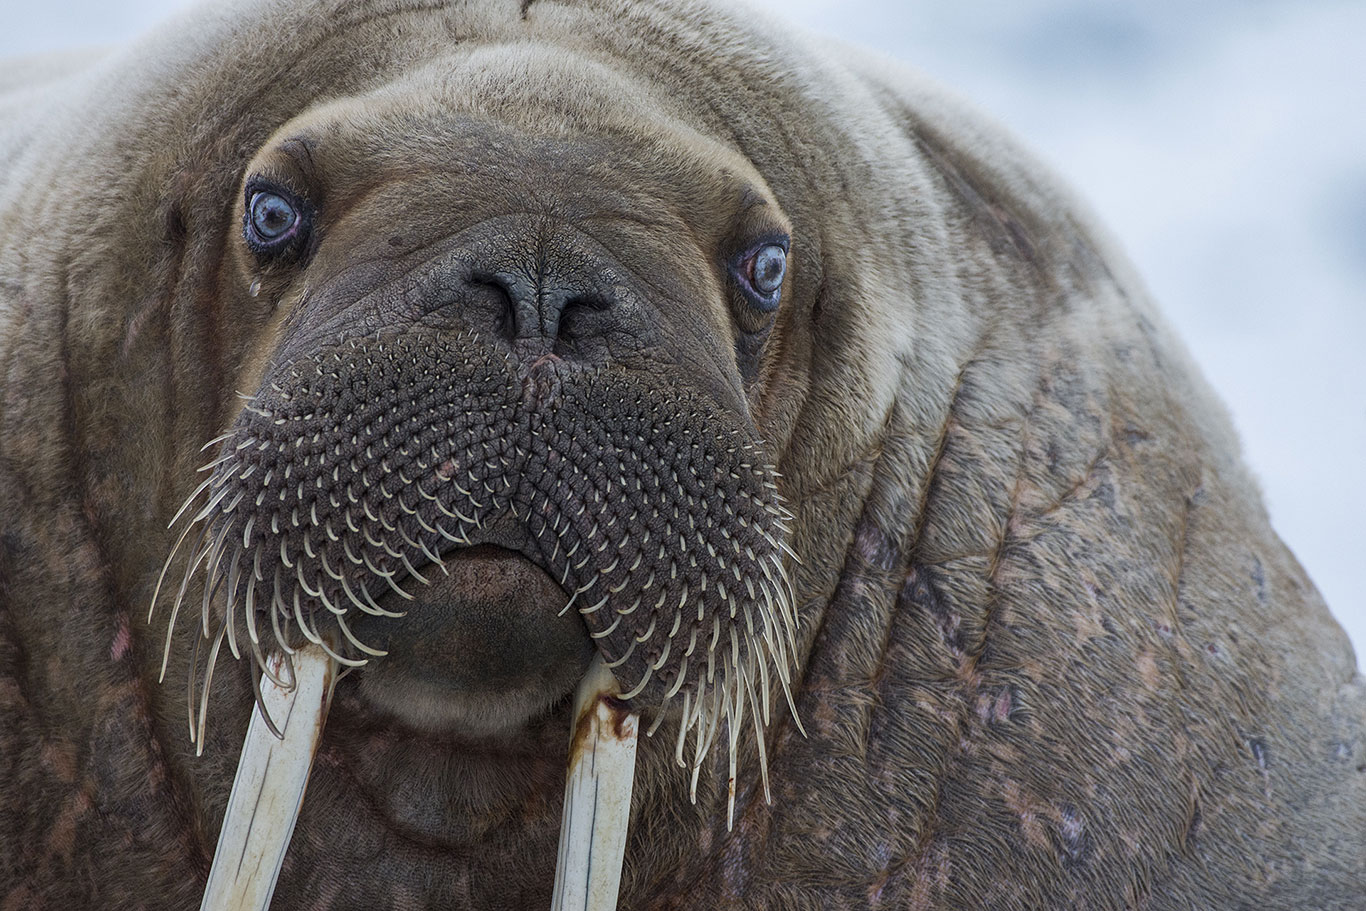
\includegraphics[scale=.3]{dimensions/phoque.jpg}
					\caption{scale $=$ \num{.3}}
				\end{subfigure}\hfill
				\begin{subfigure}{.49\linewidth}\centering
					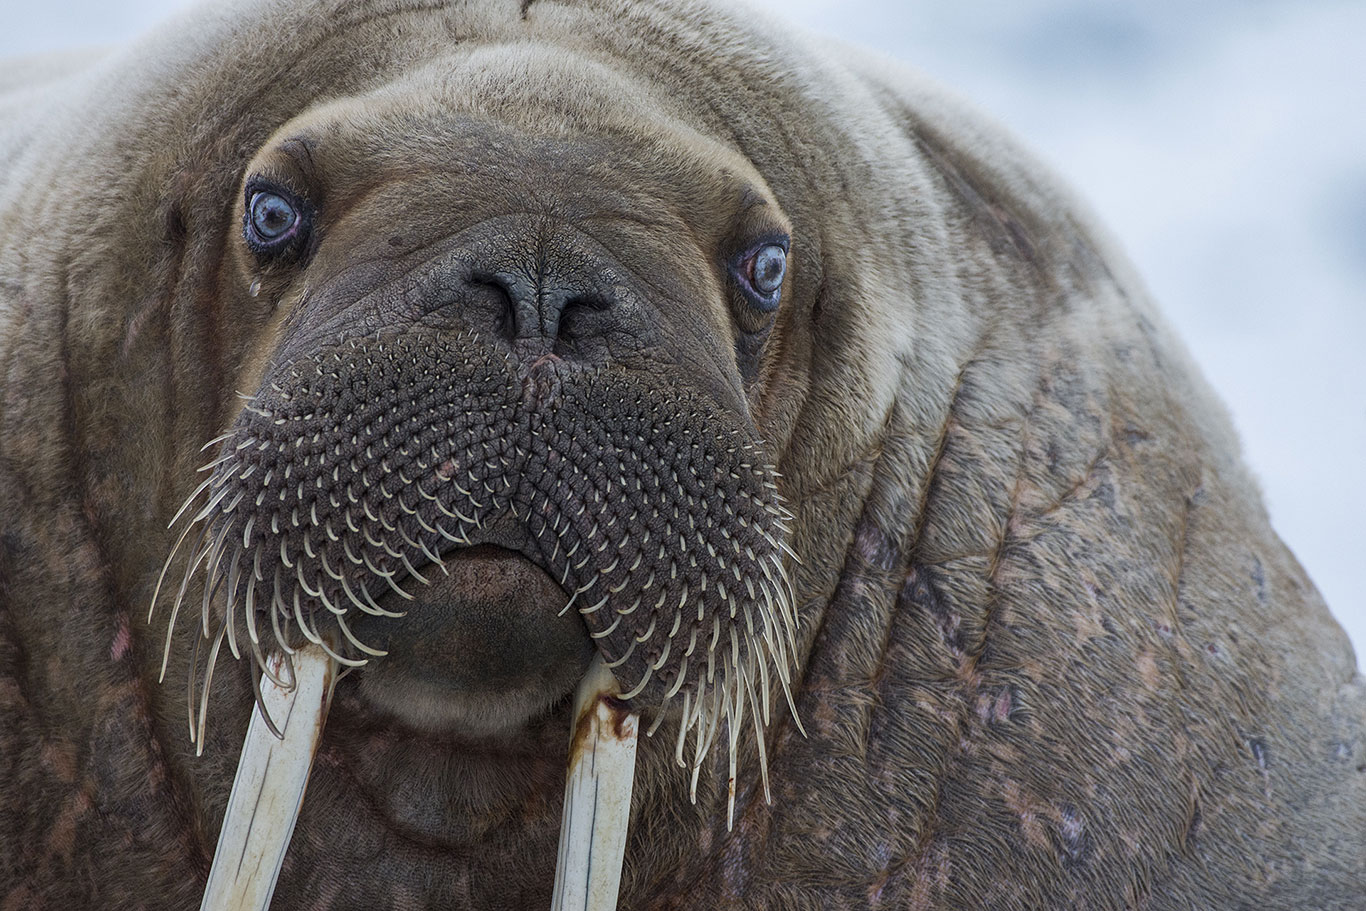
\includegraphics[scale=.1]{dimensions/phoque.jpg}
					\caption{scale $=$ \num{.1}}
				\end{subfigure}
				\caption{Effet de l'option "scale" (Attention aux tripophobes)}
			\end{figure}
			\begin{figure}[h!]\centering
				\begin{subfigure}{.49\linewidth}\centering
					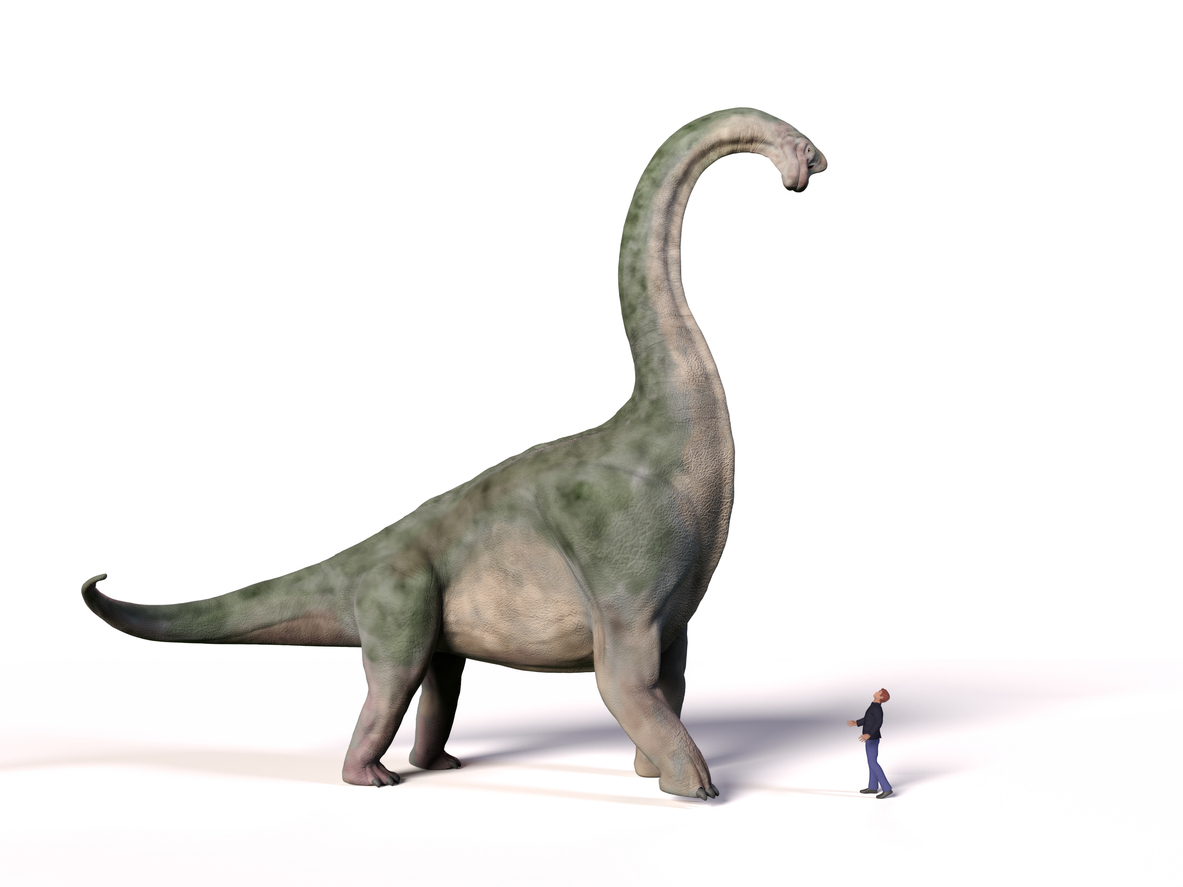
\includegraphics[height=20em]{dimensions/dinosaure.jpg}
					\caption{height $=$ \num{20}em}
				\end{subfigure}\hfill
				\begin{subfigure}{.49\linewidth}\centering
					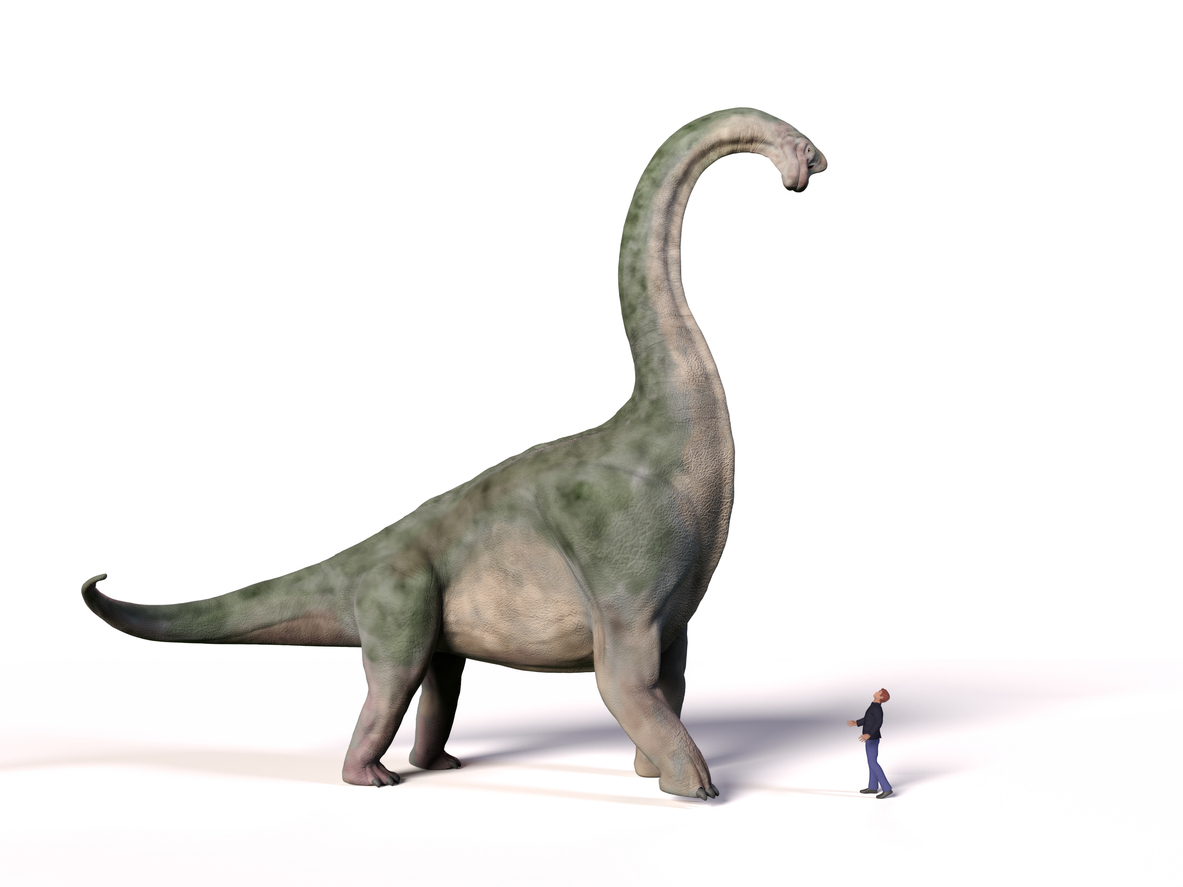
\includegraphics[height=5em]{dimensions/dinosaure.jpg}
					\caption{height $=$ \num{5}em}
				\end{subfigure}
				\caption{Effet de la définition de la hauteur}
			\end{figure}
			\begin{figure}[h!]\centering
				\begin{subfigure}{.49\linewidth}\centering
					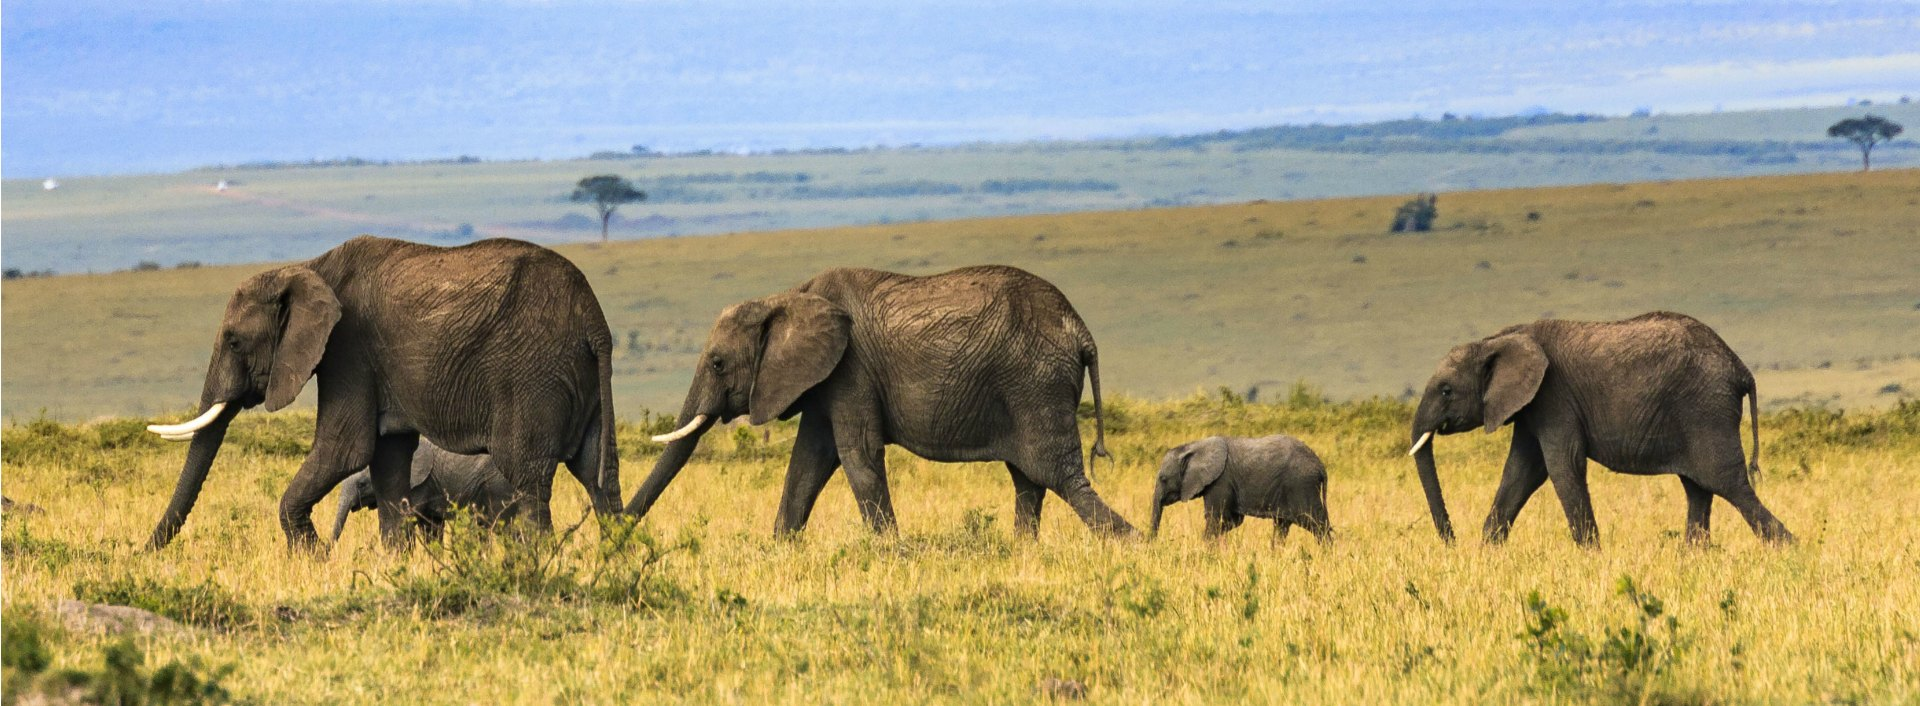
\includegraphics[width=\textwidth]{dimensions/elephants.jpg}
					\caption{width $=$ \num{0.5} textwidth}
				\end{subfigure}\hfill
				\begin{subfigure}{.49\linewidth}\centering
					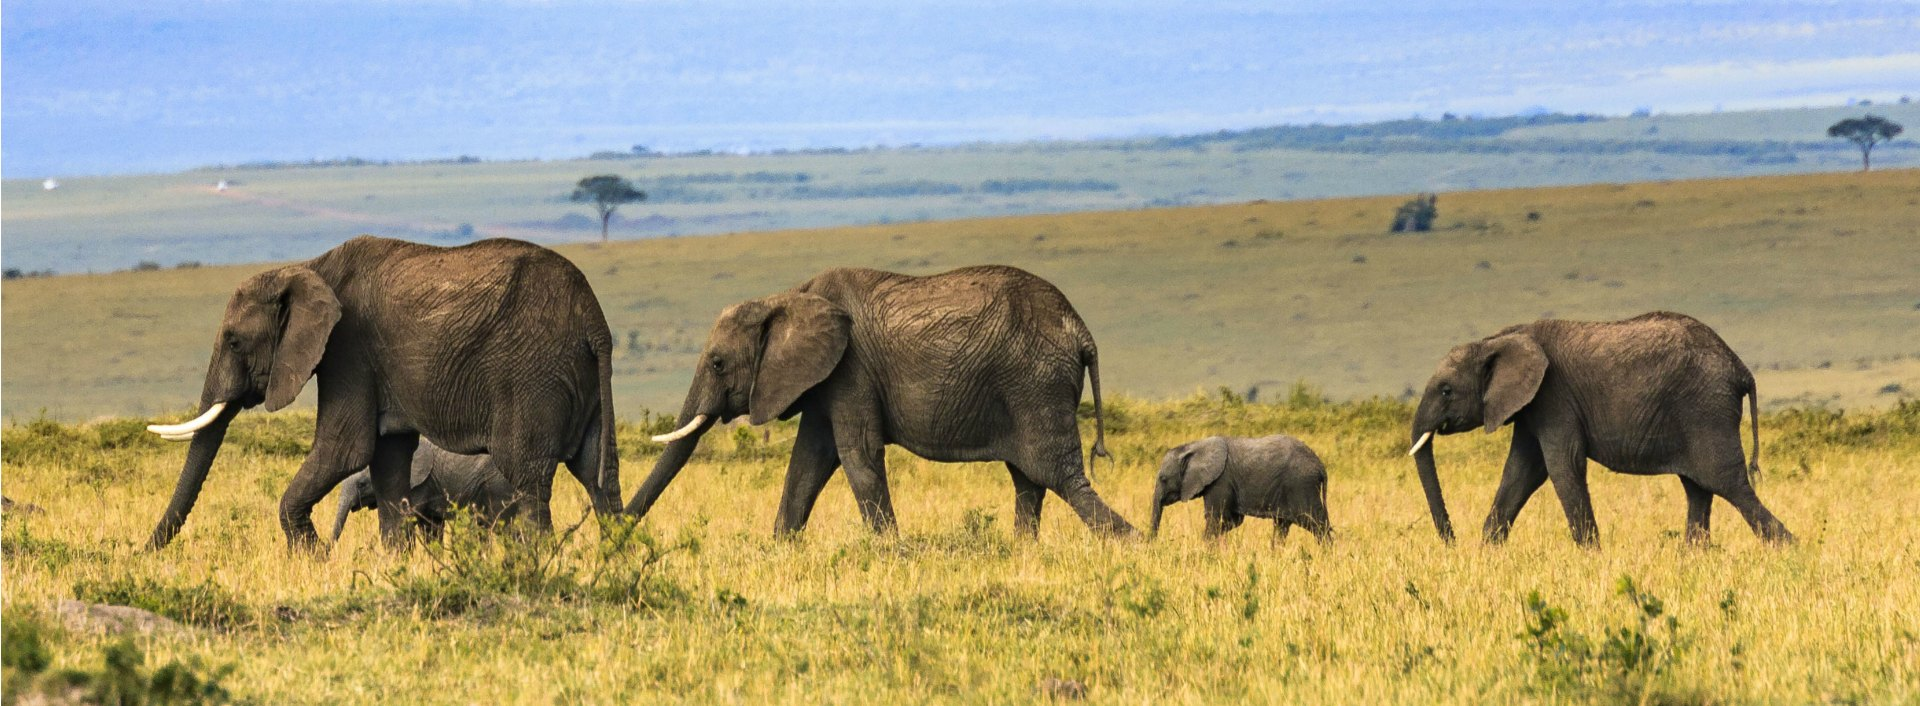
\includegraphics[width=.5\textwidth]{dimensions/elephants.jpg}
					\caption{width $=$ \num{0.25} textwidth}
				\end{subfigure}
				\caption{Effet de la définition de la largeur}
			\end{figure}
			\begin{figure}[h!]\centering
				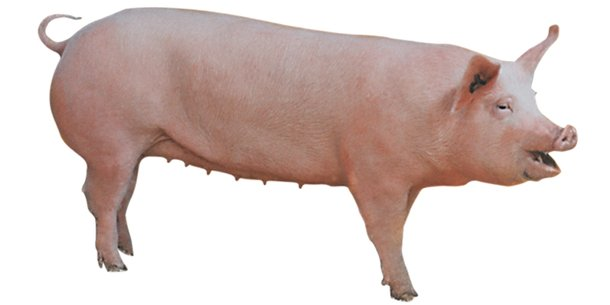
\includegraphics[height=3cm, width=\textwidth, angle=15]{dimensions/cochon.jpg}
				\caption{Association d'options : un cochon de \SI{3}{\centi\meter} de haut, long comme la largeur de la page et tourné de \SI{15}{\degree} dans le sens trigonométrique (height $=$ \SI{3}{\centi\meter}, width $=$ textwidth, angle $=$ \SI{15}{\degree}).}
			\end{figure}
	
	\chapter{Tableaux}
		L'insertion d'un tableau se fait par l'intermédiaire de l'environnement "tabular" avec un paramètre supplémentaire :
		\begin{verbatim}
			\begin{tabular}{}
				Contenu du tableau ici
			\end{tabular}
		\end{verbatim}
		\paragraph{Cool ! Et je mets quoi comme paramètre ?\\}
			Il s'agit de mentionner les colonnes. Les lignes sont ajoutées une à une dans le contenu de l'environnement. Mais avant de construire les lignes, le compilateur a besoin de connaître le nombre de colonnes, leur format et les séparateurs à utiliser. Ce paramètre donne ces informations au compilateur.
		\paragraph{... Cool ! Et je mets quoi comme paramètre ?\\}
			Au moins une lettre par colonne ("l" pour justifier le contenu à gauche, "r" pour justifier à droite ou "c" pour centrer) séparer chacune par un symbole définissant le séparateur entre les colonnes ("|" produira une ligne verticale, "||" produira une double ligne verticale, aucun séparateur n'est utilisé si rien n'est écrit).
		\paragraph{Un exemple ?\\}
			Le paramètre "rc|cl" définit un tableau de quatre colonnes : la première colonne sera justifiée à droite, les deux suivantes seront centrées et la dernière sera justifiée à gauche. Une ligne verticale est placée entre la colonne 2 et la colonne 3. Ce qui donne quelque chose comme ça :
			\begin{center}
			\begin{tabular}{rc|cl}
				Première colonne & Deuxième colonne & Troisième colonne & Quatrième colonne \\
				1 & 2 & 3 & 4
			\end{tabular}
			\end{center}
		\paragraph{Et comment on remplit les lignes ?\\}
			Pour chaque ligne, on écrit le contenu des cellules séparé par le symbole "\&" là ou le séparateur est censé être. \`A la fin de la ligne, on fait un retour de ligne "\textbackslash\textbackslash". Par exemple :
			\begin{verbatim}
			\begin{tabular}{|c|c|c|}
				Des maths & Du texte & Une image \\
				$D = 2\pi r$ & Salut ! & 
\includegraphics[width=2em]{smiley.png}
			\end{tabular}
			\end{verbatim}
			Donne :
			\begin{tabular}{|c|c|c|}
				Des maths & Du texte & Une image \\
				$D = 2\pi r$ & Salut ! & 
\includegraphics[width=2em]{smiley.png}
			\end{tabular}
		\paragraph{Et si je veux rajouter des lignes horizontales pour séparer mes lignes ?\\}
			Alors il faut faire appel à la commande "\textbackslash hline" pour ajouter une ligne horizontale complète. Si l'on veut juste une ligne horizontale du début de la colonne $i$ jusqu'à la fin de la colonne $j$ alors il faut faire appel à la commande "\textbackslash cline\{i-j\}". Par exemple :
			\begin{verbatim}
			\begin{tabular}{|c|c|c|}
				\hline
				Des maths & Du texte & Une image \\
				\cline{1-2}
				$D = 2\pi r$ & Salut ! & 
\includegraphics[width=2em]{smiley.png} \\
				\hline
			\end{tabular}
			\end{verbatim}
			Donne :
			\begin{tabular}{|c|c|c|}
				\hline
				Des maths & Du texte & Une image \\
				\cline{1-2}
				$D = 2\pi r$ & Salut ! & 
\includegraphics[width=2em]{smiley.png} \\
				\hline
			\end{tabular}
		\paragraph{Et si on souhaite écrire de longs textes dans les cellules ?\\}
			Bonne question ! En effet, \LaTeX\ dimensionne automatiquement la largeur des colonnes en fonction du contenu. Lorsqu'on veut mettre de longs textes dans une cellule alors il ne faut plus caractériser la colonne par une lettre "l", "c" ou "r" mais plutôt par le paramètre "p\{\}". La largeur de la colonne est alors donnée dans les accolades. Par exemple :
			\begin{verbatim}
			\begin{tabular}{|c|c|c|p{5cm}}
				\hline
				Des maths & Du texte & Une image & Un très long texte\\
				\cline{1-2, 4}
				$D = 2\pi r$ & Salut ! & 
\includegraphics[width=2em]{smiley.png} & \blindtext \\
				\hline
			\end{tabular}
			\end{verbatim}
			Donne :
			\begin{tabular}{|c|c|c|p{5cm}|}
				\hline
				Des maths & Du texte & Une image & Un très long texte\\
				\cline{1-2}\cline{4-4}
				$D = 2\pi r$ & Salut ! & 
\includegraphics[width=2em]{smiley.png} & \blindtext \\
				\hline
			\end{tabular}
		\paragraph{Est-ce qu'on peut changer les séparateurs verticaux ?\\}
			Oui. Grâce à la commande "\@\{\}". Il faut alors placer entre les accolades ce que l'on souhaite utiliser comme séparateur. Par exemple :\vspace{1em}\\
			\begin{minipage}[c]{.3\textwidth}
			\begin{flushright}
			\begin{verbatim}
			\begin{tabular}{r@{,}l}
				3 & 14159 \\
				98 & 20 \\ \hline
				101 & 34159
			\end{tabular}
			\end{verbatim}
			\end{flushright}
			\end{minipage}
			\begin{minipage}[c]{.59\textwidth}
			Donne :
			\begin{tabular}{r@{,}l}
				3 & 14159 \\
				98 & 20 \\ \hline
				101 & 34159
			\end{tabular}
			\end{minipage}

	\chapter{Positionner et labelliser les flottants}
		Maintenant que nous savons plus ou moins insérer des images et des tableaux, il est possible de jouer avec les flottants associés. Pour rappel, les flottants associés aux figures et aux tableaux seront, respectivement, dans des environnements "figure" et "table". Il suffit donc d'insérer les images et tableaux dans leur environnement respectif et \LaTeX\ se charge de la numérotation automatique et de la mise en forme. Cela comprend également la possibilité d'insérer une "Table des figures" et une "Liste des tableaux" dans le document.
		\paragraph{Très bien mais il se met où dans le document le flottant ?\\}
			Son point d'ancrage est toujours là où il est écrit dans le code \LaTeX . Par contre, afin de respecter les normes les plus usuelles, \LaTeX\ fait en sorte de placer les flottants plutôt en haut ou en bas de page. Lorsqu'il y a beaucoup de flottants qui se suivent, le programme fait en sorte de les rassembler sur une ou plusieurs pages dédiée(s) à leur affichage.\\\indent
			Faisons un premier essai : j'insère une image flottante juste ici. [Je l'ai fais, promis !]
			\begin{figure}\centering
				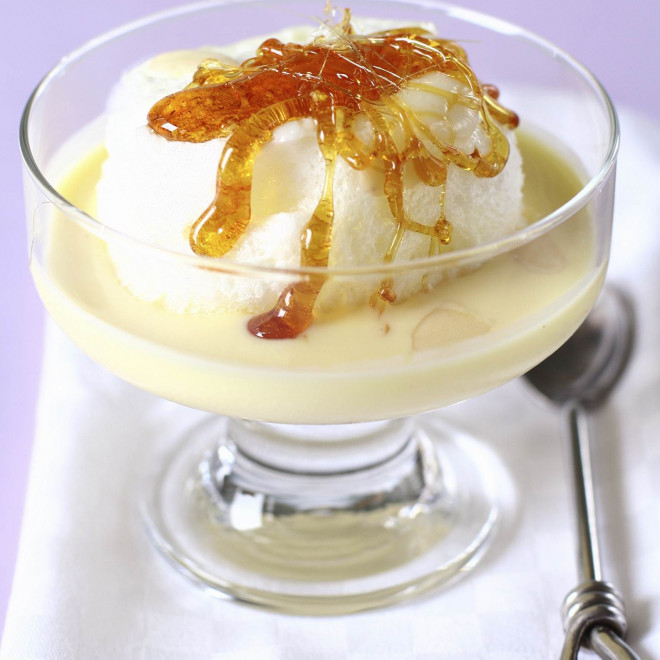
\includegraphics[width=.3\textwidth]{positions/flottante.jpg}
				\caption{Une image flottante ... heuuuu... Une île flottante !}
			\end{figure}
			Ce texte est écrit après l'insertion du flottant et se retrouve pourtant à la suite du texte précédent. Même avec les paragraphes qui suivent, l'image restera en bas de cette page.
		\paragraph{Et si je veux choisir où placer mon flottant ?\\}
			Pas de problème ! Il faut juste savoir que \LaTeX\ fera de son mieux pour faire ce que l'on veut mais n'y arrive pas toujours. Assez souvent, on lui demande des choses impossibles. Pour rappel, un flottant n'est pas dissociable, on ne peut donc pas lui demander de tenir sur la même page que le texte si cela ne rentre pas. Pour mentionner notre préférence de placement, il suffit de la préciser entre crochets juste après l'appel de l'environnement. La position se fait à l'aide d'une lettre : "t" pour dire "en-haut", "b" pour dire "en-bas" et "h" pour dire "ici". Par exemple, \verb|\begin{figure}[t]...| veut dire "Essaies de faire le maximum pour placer l'image en haut de page". Cela est illustré sur la page suivante.
		\paragraph{Est-ce que mes préférences de placement sont toujours respectées ?\\}
			Elles ne le sont pas si cela est impossible. Elles ne le sont pas également quand le résultat est considéré comme non-élégant. Il est alors possible de forcer \LaTeX\ à le faire en ajoutant un point d'exclamation. Par exemple, \verb|\begin{figure}[h!]...| dit à \LaTeX\ "Eh oh ! Tu m'écoutes et tu fais ce que je te dis dans la limite du possible ! Tu mets cette image ici !".
		
		\newpage
		\paragraph{Voici un texte mentionnant une image placée en haut de page\\}
			Cette phrase est écrite avant d'ajouter l'image de haut de page (fig \ref{fig:haut1}).
			\begin{figure}[t]\centering
				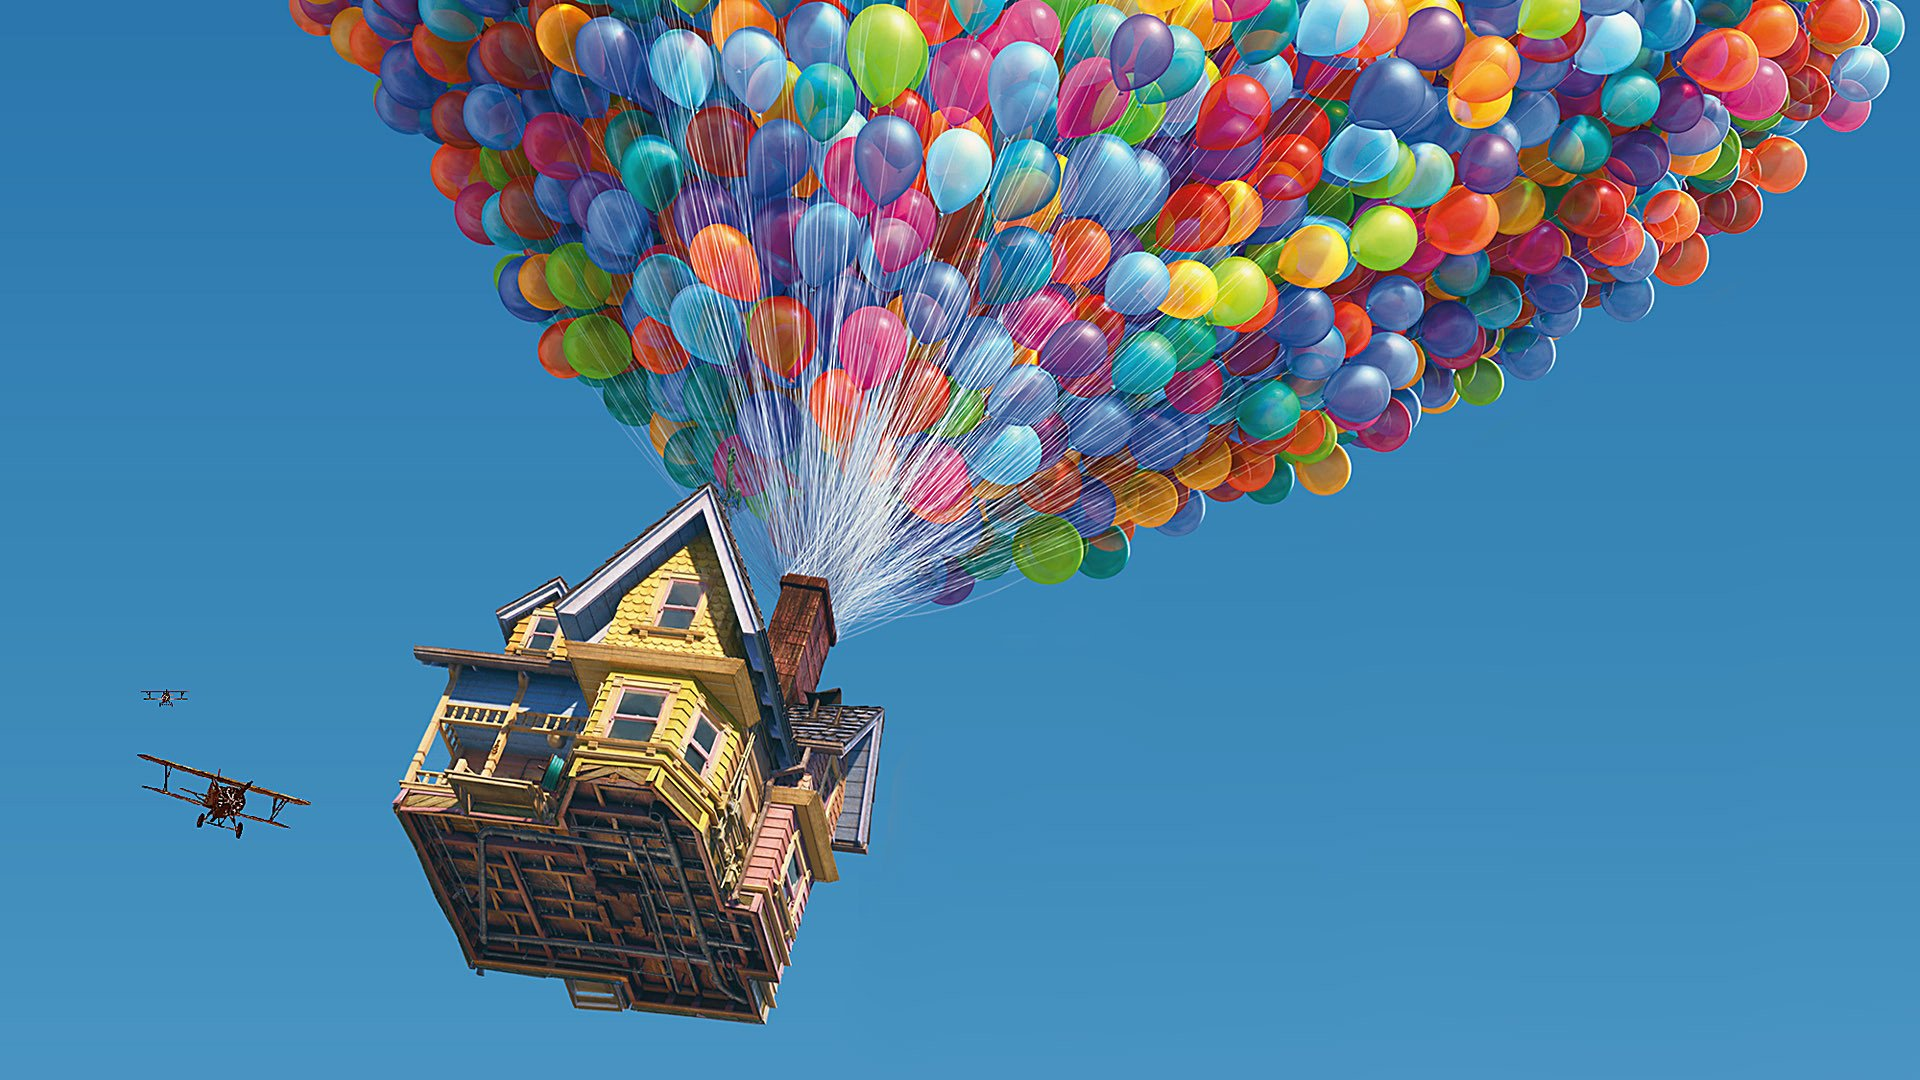
\includegraphics[width=.5\textwidth]{positions/haut.jpg}
				\caption{\label{fig:haut1}Haut les ballons !}
			\end{figure}
			\\Je viens de placer l'image. Ce texte vient donc après.
		\paragraph{Voici un texte mentionnant une image placée à l'endroit exact\\}
			Cette phrase est écrite avant d'ajouter l'image juste ici  (fig \ref{fig:ici1}).
			\begin{figure}[h]\centering
				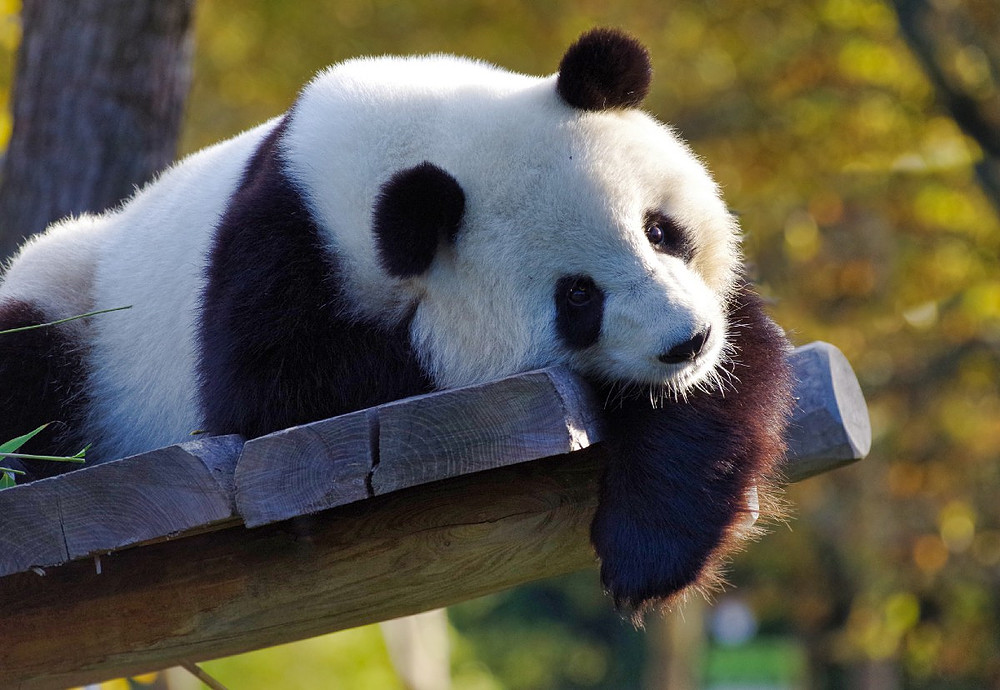
\includegraphics[width=.4\textwidth]{positions/where_i_want.jpg}
				\caption{\label{fig:ici1}On est bien ici...}
			\end{figure}
			\\Je viens de placer l'image. Ce texte vient donc après.
		\paragraph{Voici un texte mentionnant une image placée en bas de page\\}
			Cette phrase est écrite avant d'ajouter l'image en bas de page (fig \ref{fig:bas1}).
			\begin{figure}[b]\centering
				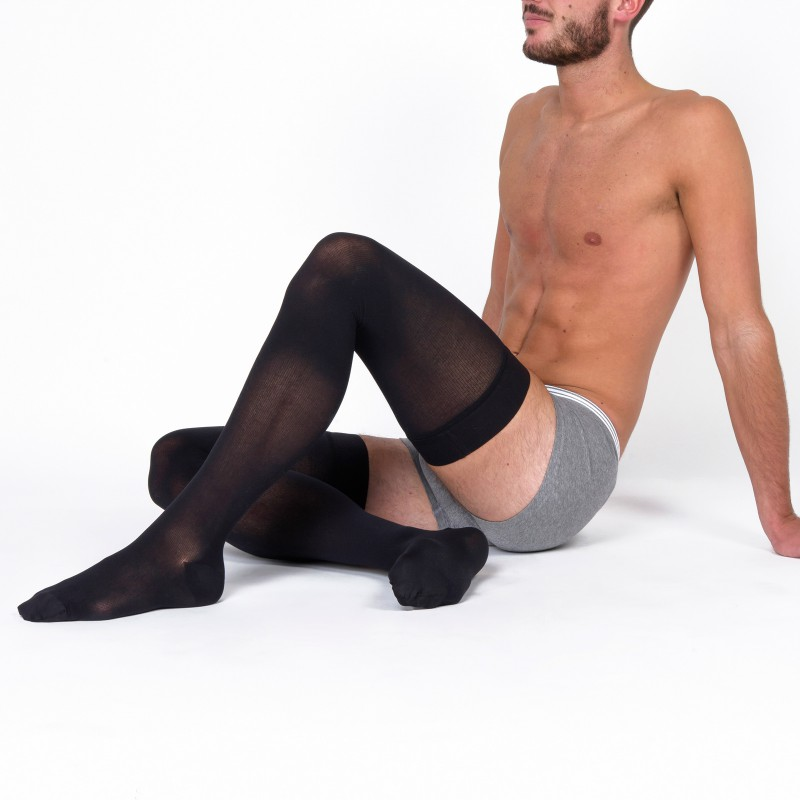
\includegraphics[width=.35\textwidth]{positions/bas.jpg}
				\caption{\label{fig:bas1}On est bien en bas également...}
			\end{figure}
			\\Je viens de le faire. Ce texte vient donc après.
			
		\newpage
		\paragraph{Même page sans mentionner les préférences de placement}
		\paragraph{Voici un texte mentionnant l'image initialement placée en haut de page\\}
			Cette phrase est écrite avant d'ajouter l'image de haut de page (fig \ref{fig:haut2}).
			\begin{figure}\centering
				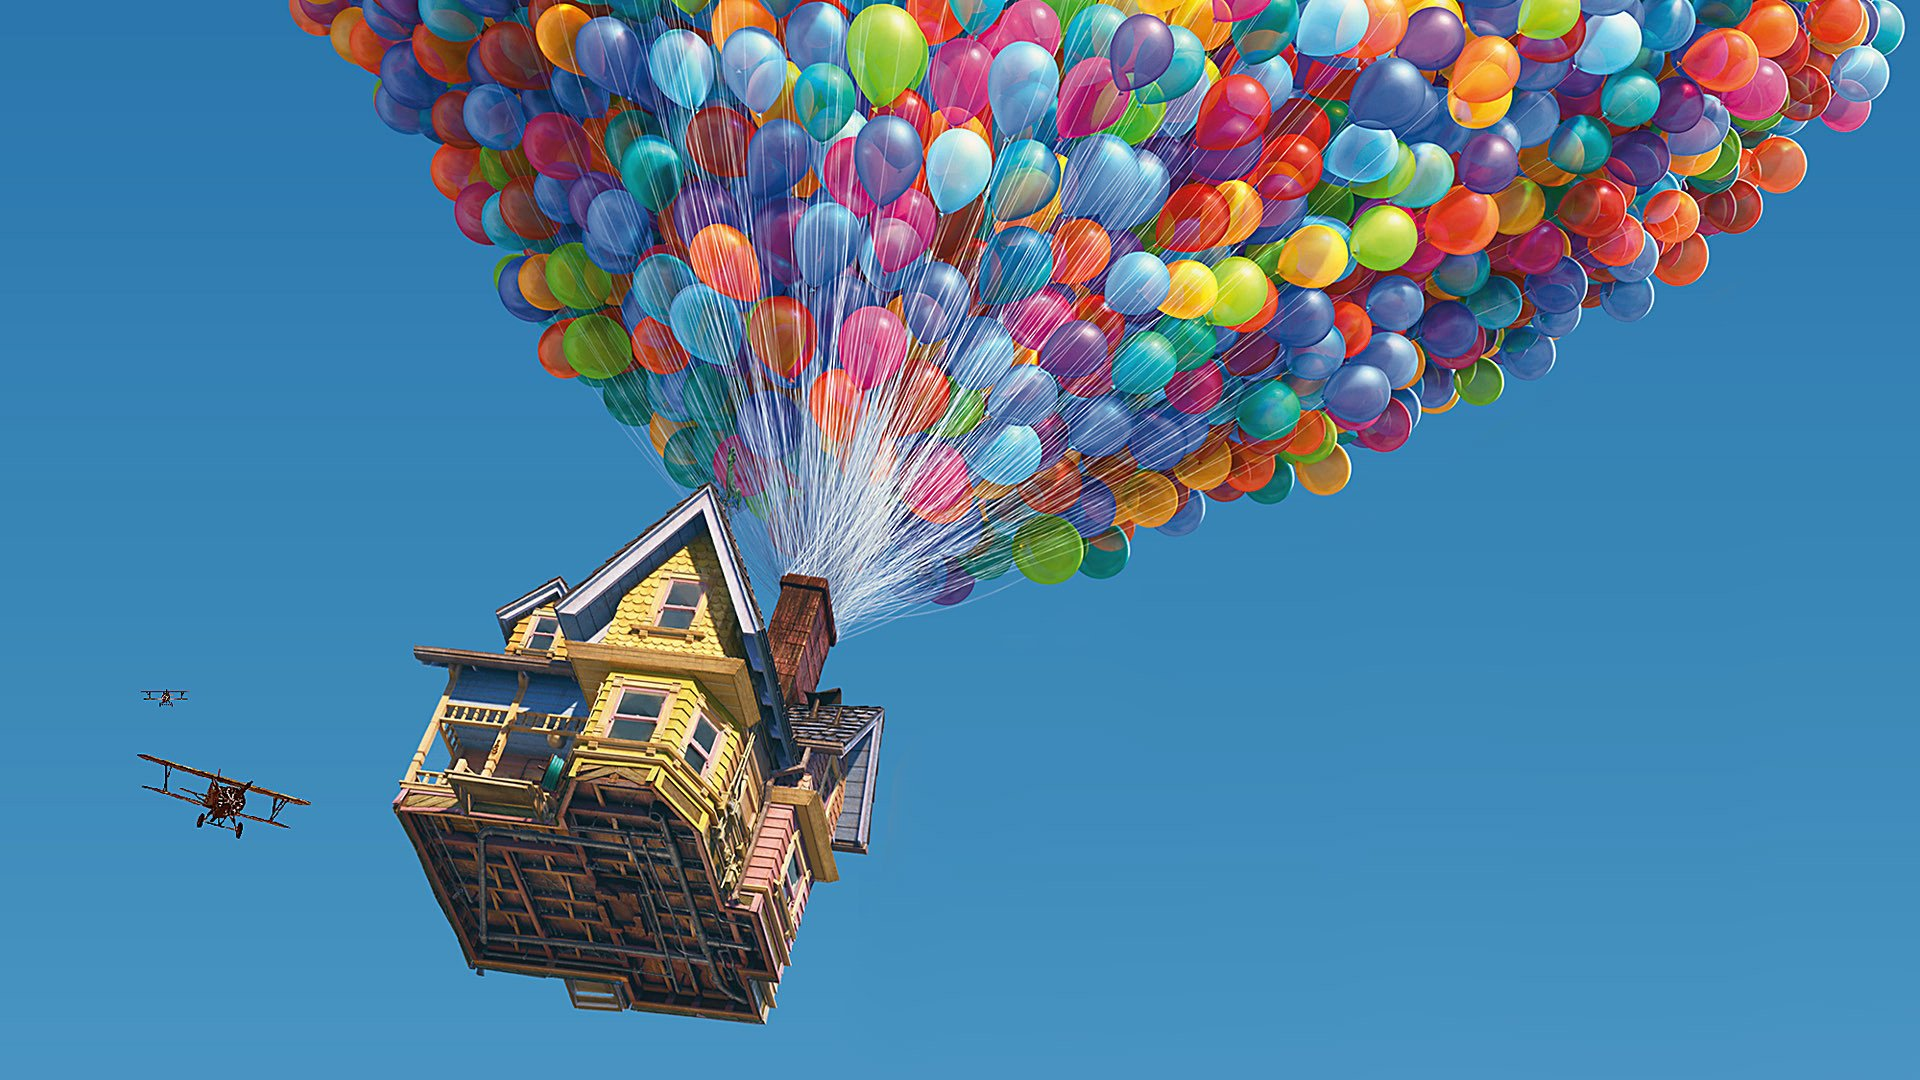
\includegraphics[width=.5\textwidth]{positions/haut.jpg}
				\caption{\label{fig:haut2}Haut les ballons !}
			\end{figure}
			\\Je viens de placer l'image. Ce texte vient donc après.
		\paragraph{Voici un texte mentionnant l'image initialement placée à l'endroit exact\\}
			Cette phrase est écrite avant d'ajouter l'image juste ici (fig \ref{fig:ici2}).
			\begin{figure}\centering
				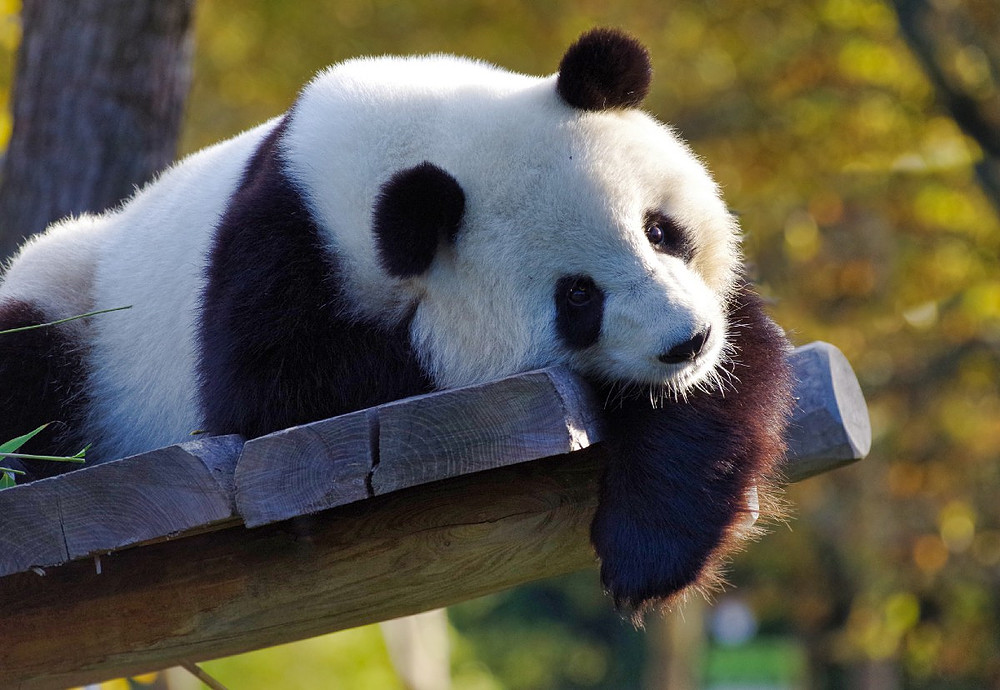
\includegraphics[width=.4\textwidth]{positions/where_i_want.jpg}
				\caption{\label{fig:ici2}On est bien ici...}
			\end{figure}
			\\Je viens de placer l'image. Ce texte vient donc après.
		\paragraph{Voici un texte mentionnant l'image initialement placée en bas de page\\}
			Cette phrase est écrite avant d'ajouter l'image en bas de page (fig \ref{fig:bas2}).
			\begin{figure}\centering
				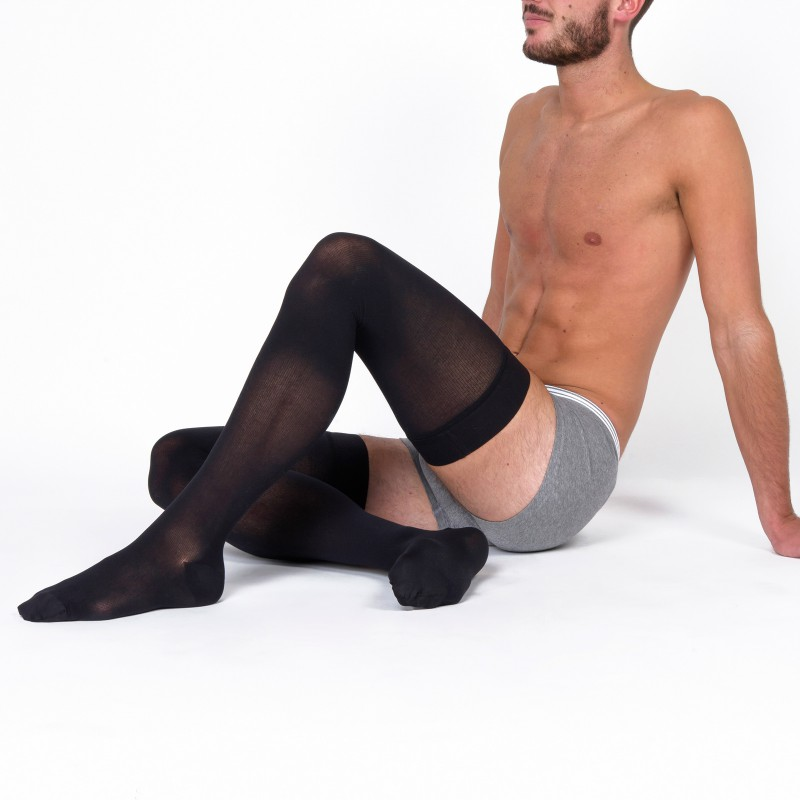
\includegraphics[width=.35\textwidth]{positions/bas.jpg}
				\caption{\label{fig:bas2}On est bien en bas également...}
			\end{figure}
			\\Je viens de le faire. Ce texte vient donc après.
			
		\newpage
		\paragraph{Tout ça c'est bien mais comment tu as centré horizontalement tes flottants ?\\}
			Pour cela, il suffit de rajouter la commande "\textbackslash centering" dès le début de l'environnement. Cela centrera tout ce qui se trouve dans l'environnement, pas en dehors.
			\begin{verbatim}
				\begin{figure}[h]
					
\includegraphics[width=.3\textwidth]{gauche.jpg}
					\caption{Une image alignée comme le texte (à gauche)}
				\end{figure}
			\end{verbatim}
			Affiche :
			\begin{figure}[h]
				
\includegraphics[width=.3\textwidth]{gauche.jpg}
				\caption{Une image alignée comme le texte (à gauche)}
			\end{figure}
			\\Alors que
			\begin{verbatim}
				\begin{figure}[h]\centering
					
\includegraphics[width=.6\textwidth]{chuck_norris.jpg}
					\caption{Si Dieu le peut, Chuck le peut. Nous aussi...}
				\end{figure}
			\end{verbatim}
			Affiche :
			\begin{figure}[h]\centering
				
\includegraphics[width=.6\textwidth]{chuck_norris.jpg}
				\caption{Si Dieu le peut, Chuck le peut. Nous aussi...}
			\end{figure}
		
		\newpage
		\paragraph{Et la légende dans tout ça ?\\}
			Il ne reste plus que ça à voir en effet. Il suffit de rajouter la commande "\textbackslash caption\{\}" dans le flottant. Le texte situé à l'intérieur de la commande sera le texte de la légende. Par exemple :
			\begin{verbatim}
				\begin{figure}[h]\centering
					
\includegraphics[width=.5\textwidth]{legende.jpg}
					\caption{Je suis la légende de l'affiche "Je suis une légende"}
				\end{figure}
			\end{verbatim}
			affiche :
			\begin{figure}[h]\centering
				
\includegraphics[width=.5\textwidth]{legende.jpg}
				\caption{Je suis la légende de l'affiche "Je suis une légende"}
			\end{figure}
		\paragraph{Comment faire un renvoi vers un flottant dans texte ?\\}
			Dans le texte, il est nécessaire de faire appel à une référence avec la commande "\textbackslash ref\{\}". L'argument pris en paramètre est un identifiant unique permettant de retrouver le bon flottant. En contre partie, il est nécessaire de mentionner cette référence unique dans le flottant considéré grâce à la commande "\textbackslash label\{\}". La pratique veut que l'on place la commande "label" à l'intérieur de la légende. Par exemple :
			\begin{verbatim}
				\subparagraph{}Mon image est visible sur la figure \ref{fig:maref} à la page \pageref{fig:maref}.
				\begin{figure}[h]\centering
					
\includegraphics[width=.5\textwidth]{renvoye.jpg}
					\caption{\label{fig:maref}Je me suis fait renvoyé !}
				\end{figure}
			\end{verbatim}
			Affiche :\\
			\subparagraph{}Mon image est visible sur la figure \ref{fig:maref} à la page \pageref{fig:maref}.
				\begin{figure}[h]\centering
					
\includegraphics[width=.5\textwidth]{renvoye.jpg}
					\caption{\label{fig:maref}Je me suis fait renvoyé !}
				\end{figure}
	
	\chapter{Sous-figures et sous-tableaux}
		
	
	\chapter{Environnement minipage et "spacer"}
		
	
\end{document}
